% TeX root = ../main.tex
\newpage
\section{Toán hình khối}
Ngoài việc sử dụng nhuần nhuyễn các công thức ta cần phải luyện tập thêm khả năng tưởng tượng hình khối trong không gian.
\xd 
\textbf{Hình trụ:}
\[
    \begin{cases}
        V_\textit{hình trụ} = S_\textit{đáy~} . \textit{~cao} = \pi . R^2 . h \\[0.5em]
        S_{xq~\textit{hình trụ}} = C_\textit{đáy~} . \textit{~cao} = 2\pi Rh
    \end{cases}
\]
\xd
\textbf{Hình nón:}
\[
    \begin{cases}
        V_\textit{hình nón} =\frac{1}{3}~.~ S_\textit{đáy~} . \textit{~cao} = \frac{1}{3}.\pi . R^2 . h \\[0.5em]
        S_{xq~\textit{hình nón}} = \pi . R . l
    \end{cases}
\]
\xd
\textbf{Hình cầu:}
\[
    \begin{cases}
        V_\textit{hình cầu} = \frac{4}{3}.\pi . R^3 \\[0.5em]
        S_{xq~\textit{hình cầu}} = 4.\pi . R^2 
    \end{cases}
\]
\xd
\textbf{Hình hộp chữ nhật:}
\[
    \begin{cases}
        V_\textit{hình hộp chữ nhật} = S_\textit{đáy~} . \textit{~cao} = \textit{dài~}.\textit{~rộng~}.\textit{~cao} \\[0.5em]
        S_{xq~\textit{hình hộp chữ nhật}} = C_\textit{đáy~} . \textit{~cao} = 2.(\textit{dài + rộng}).\textit{~cao}
    \end{cases}
\]
\xd
\textbf{Hình lập phương:}
\[
    \begin{cases}
        V_\textit{hình lập phương} = \textit{cạnh}^3 \\[0.5em]
        S_{xq~\textit{hình lập phương}} = 6.\textit{cạnh}^2
    \end{cases}
\]

\begin{marginfigure}|-11cm|
	\centering
	\includegraphics[width=0.6\marginparwidth]{imgc2/3-4/hinh_tru.pdf}
    \vspace{0.2cm}
	\margincaption{Hình trụ}
\end{marginfigure}

\begin{marginfigure}|-7cm|
	\centering
	\includegraphics[width=0.6\marginparwidth]{imgc2/3-4/hinh_non.pdf}
    \vspace{0.2cm}
	\margincaption{Hình nón}
\end{marginfigure}

\begin{marginfigure}|-7cm|
	\centering
	\includegraphics[width=0.6\marginparwidth]{imgc2/3-4/hinh_cau.pdf}
    \vspace{0.2cm}
	\margincaption{Hình cầu}
\end{marginfigure}

\begin{marginfigure}|-7cm|
	\centering
	\includegraphics[width=0.6\marginparwidth]{imgc2/3-4/hop_cn.pdf}
    \vspace{0.2cm}
	\margincaption{Hình hộp chữ nhật}
\end{marginfigure}

\begin{marginfigure}|-7cm|
	\centering
	\includegraphics[width=0.6\marginparwidth]{imgc2/3-4/lap_phuong.pdf}
    \vspace{0.2cm}
	\margincaption{Hình lập phương}
\end{marginfigure}
\newpage
\begin{smallfont}
    \bt[TUYỂN SINH HỒ CHÍ MINH 2025-2026]
    {
        Một hộp đựng bóng tennis có dạng hình trụ chứa vừa khít 4 quả bóng tennis có dạng hình cầu như hình. Biết diện tích bề mặt mỗi quả bóng tennis là $132,67~cm^2$.
        \begin{enumerate}[label=\alph*)]
            \item Tính bán kính mỗi quả bóng tennis.
            \item Nhà sản xuất thường sử dụng các thùng giấy hình hộp chữ nhật (có nắp) để chứa 12 hộp tennis sao cho các hộp tennis được xếp vừa khít trong thùng giấy như hình. Hỏi cần tối thiểu bao nhiêu $m^2$ giấy để thiết kế một thùng như trên (giả sử các mép nối không đáng kể).
        \end{enumerate}
    }
    % Hình
    \begin{marginfigure}|-3.5cm|
        \centering
        \includegraphics[width=\marginparwidth]{imgc2/3-4/HCM2526.pdf}
        \vspace{-0.2cm}
        \margincaption{Bài 1}
    \end{marginfigure}
    \xdd 
    \bt[TUYỂN SINH HỒ CHÍ MINH 2024-2025]
    {
        Anh Huy là một nghệ nhân và anh đang thiết kế một mô hình Trái đất dạng hình cầu có thể tích $4,2~dm^3$.
        \begin{enumerate}[label=\alph*)]
            \item Tìm bán kính của mô hình Trái đất mà anh Huy thiết kế (kết quả làm tròn đến hàng đơn vị). 
            \item Anh Huy dự định làm một cái hộp bằng giấy (bao gồm cả nắp hộp) để đựng mô hình Trái đất (như hình vẽ trên). Anh đang phân vân nên làm hộp hình lập phương hay hộp hình trụ thì tốn ít giấy hơn. Hãy cho biết anh Huy nên chọn phương án nào? Biết các mặt hộp đều tiếp xúc với mô hình Trái đất và lượng giấy phát sinh là không đáng kể.
        \end{enumerate} 
    }
    % Hình
    \begin{marginfigure}|-4.5cm|
        \centering
        \includegraphics[width=\marginparwidth]{imgc2/3-4/HCM2425.pdf}
        \margincaption{Bài 2}
    \end{marginfigure}
    \xdd 
    \bt[TUYỂN SINH HỒ CHÍ MINH 2023-2024]
    {
        Bạn Nam dự định tổ chức buổi tiệc sinh nhật và chọn loại ly có phần chứa nước dạng hình nón với bán kính đáy $R = 4~cm$ và độ dài đường sinh $l = 10~cm$ để khách uống nước trái cây.
        \begin{enumerate}[label=\alph*)]
            \item Tính thể tích phần chứa nước của ly (kết quả làm tròn đến hàng đơn vị).
            \item Bạn Nam cần chuẩn bị một số hộp nước trái cây có lượng nước trong mỗi hộp là 1,2 lít. Biết rằng buổi tiệc sinh nhật có 14 người (đã bao gồm Nam). Nếu mỗi người trung bình uống 3 ly nước trái cây và lượng nước rót bằng 90\% thể tích ly thì bạn Nam cần chuẩn bị ít nhất bao nhiêu hộp nước trái cây?
        \end{enumerate}
    }
    % Hình
    \begin{marginfigure}|-5.5cm|
        \centering
        \includegraphics[width=0.4\marginparwidth]{imgc2/3-4/HCM2324.pdf}
        \vspace{0.4cm}
        \margincaption{Bài 3}
    \end{marginfigure}
    \xdd 
    \bt[TUYỂN SINH HỒ CHÍ MINH 2022-2023]
    {
        Một đống cát dạng hình nón có chu vi đáy là $25,12~m$ và độ cao là $1,5~m$.
        \begin{enumerate}[label=\alph*)]
            \item Tính thể tích đống cát trên?
            \item Người ta dùng xe cải tiến để vận chuyển đống cát đó đến khu vực xây dựng. Biết thùng của xe cải tiến có dạng hình hộp chữ nhật có kích thước dài $1~m$, rộng $6~dm$ và cao $3~dm$. Trong mỗi chuyến xe, thùng xe có thể chứa nhiều hơn thể tích thực của nó là $10\%$ để vận chuyển được nhiều cát hơn. Hỏi cần ít nhất bao nhiêu chuyến xe cải tiến để chuyển hết đống cát trên?
        \end{enumerate}
    }
    % Hình
    \begin{marginfigure}|-3.5cm|
        \centering
        \includegraphics[width=\marginparwidth]{imgc2/3-4/HCM2223.pdf}
        %\vspace{}
        \margincaption{Bài 4}
    \end{marginfigure}
    \xdd 
    \bt[TUYỂN SINH HỒ CHÍ MINH 2020-2021]
    {
        Anh Minh vừa mới xây một cái hồ trữ nước cạnh nhà có hình dạng hộp chữ nhật kích thước $2~m \times 2~m \times 1~m$. Hiện hồ chưa có nước nên anh Minh phải ra sông lấy nước. Mỗi lần ra sông anh gánh được 1 đôi nước đầy gồm 2 thùng hình trụ bằng nhau có bán kính đáy $0,2~m$, chiều cao $0,4~m$.
        \begin{enumerate}[label=\alph*)]
            \item Tính lượng nước ($m^3$) anh Minh đổ vào hồ sau mỗi lần gánh (ghi kết quả làm tròn đến 2 chữ số thập phân). Biết trong quá trình gánh nước về thì lượng nước bị hao hụt khoảng $10\%$
            \item Hỏi anh Minh phải gánh ít nhất bao nhiêu lần để đầy hồ? Bỏ qua thể tích thành hồ.
        \end{enumerate}
    }
    % Hình
    \begin{marginfigure}|-3cm|
        \centering
        \includegraphics[width=0.5\marginparwidth]{imgc2/3-4/HCM2021.pdf}
        \vspace{0.4cm}
        \margincaption{Bài 5}
    \end{marginfigure}
    \xdd 
    \bt[TUYỂN SINH TRÀ VINH 2025-2026]
    {
        Một cái ly hình trụ có bán kính đáy là $7~cm$, chiều cao là $18~cm$ (bỏ qua bề dày của thành ly).
        \begin{enumerate}[label=\alph*)]
            \item Tính thể tích của cái ly.
            \item Cái ly đang chứa nước. Khối lượng nước bên trong ly có dạng hình trụ chiều cao $10~cm$. Người ta thả từ từ từng viên bi hình cầu làm bằng thép đặc (không thấm nước) có bán kính $3~cm$ vào trong ly. Hỏi có thể thả nhiều nhất bao nhiêu viên bi ngập hoàn toàn để nước dâng lên tối đa mà không bị tràn ra ngoài?
        \end{enumerate}
    }
    % Hình
    \begin{marginfigure}|-6cm|
        \centering
        \includegraphics[width=\marginparwidth]{imgc2/3-4/TV2526.pdf}
        %\vspace{}
        \margincaption{Bài 6}
    \end{marginfigure}
    \xdd 
    \bt[TUYỂN SINH ĐỒNG NAI 2025-2026]
    {
        Một chiếc mũ chú hề được làm bằng giấy gốm phần vành mũ có dạng hình vành khuyên giới hạn bởi đường tròn lớn và đường tròn nhỏ có bán kính lần lượt là $22~cm$ và $10~cm$; phần thân mũ có dạng hình nón, không đáy, gắn vào vành mũ (đường tròn đáy của thân mũ trùng với đường tròn nhỏ của vành mũ) và có độ dài đường sinh bằng $36~cm$ (xem hình bên).
    }
    % Hình
    \begin{marginfigure}|-5cm|
        \centering
        \includegraphics[width=0.75\marginparwidth]{imgc2/3-4/DN2526.pdf}
        \vspace{0.4cm}
        \margincaption{Bài 7}
    \end{marginfigure}
    \xdd 
    \bt[TUYỂN SINH KIÊN GIANG 2025-2026]
    {
        Một dụng cụ trộn bê tông có dạng một phần hình trụ và một phần hình nón, không có nắp (Hình dụng cụ và các kích thước cho như hình vẽ). Tính tiền công phải trả để sơn hết mặt ngoài của dụng cụ? Biết rằng tiền công sơn $1~m^2$ có giá $200~000$ đồng. (Lấy $\pi$ = 3,14)
    } 
    % Hình
    \begin{marginfigure}|-3cm|
        \centering
        \includegraphics[width=0.7\marginparwidth]{imgc2/3-4/KG2526.pdf}
        \vspace{0.4cm}
        \margincaption{Bài 8}
    \end{marginfigure}
    \xdd
    \bt[TUYỂN SINH NGHỆ AN 2025-2026]
    {
        \begin{enumerate}[label=\alph*)]
            \item Một bác nông dân có một bình đựng nước chè xanh, phần chứa nước là dạng hình trụ có bán kính đáy bằng $4~cm$, mực nước trong bình có chiều cao bằng $10~cm$. Bác muốn đổ hết nước từ bình sang một cái bát uống nước, phần chứa nước là dạng nửa hình cầu có bán kính bằng $6~cm$ (hình vẽ bên). Hỏi nếu đổ như vậy thì nước có bị tràn ra ngoài hay không? Vì sao?
            \item Một công ty bánh kẹo muốn sản xuất một loại kẹo có dạng hình nón. Nhân của kẹo làm bằng sô cô la là một hình trụ có bán kính đáy và chiều cao cùng bằng $1~cm$, một đáy của nhân kẹo nằm trên mặt đáy của hình nón và có tâm trùng với tâm đáy hình nón, đường tròn đáy còn lại của hình trụ nằm trên mặt xung quanh của hình nón. Phần còn lại của kẹo được phủ đầy bằng sữa khô (hình vẽ bên). Biết rằng công ty đã thiết kế viên kẹo có thể tích nhỏ nhất để tiết kiệm tối đa nguyên liệu sữa khô. Tính chiều cao của viên kẹo.
        \end{enumerate}
        % Hình
        \begin{center}
		    \includegraphics[width=0.45\textwidth]{imgc2/3-4/NA2526a.pdf}\hfill
		    \includegraphics[width=0.4\textwidth]{imgc2/3-4/NA2526b.pdf}\hfill
            \captionsetup{hypcap=false}
		    \captionof{figure}{Bài 9a; 9b}
        \end{center}
    }
    % Hình
    \begin{marginfigure}
        \centering
        \includegraphics[width=0.8\marginparwidth]{imgc2/3-4/QN2526.pdf}
        \vspace{0.4cm}
        \margincaption{Bài 10}
    \end{marginfigure}
    \xdd 
    \bt[TUYỂN SINH QUẢNG NGÃI 2025-2026]
    {
        Bác Hoa mua một thúng muối vun đầy, cái thúng có dạng nửa hình cầu với đường kính $48~cm$, phần muối vun lên có dạng hình nón với chiều cao $14~cm$ (hình vẽ bên). Bác Hoa cần phải sử dụng ít nhất bao nhiêu thùng nhựa như trên để đựng hết lượng muối đã mua. (Bỏ qua bề dày của thùng nhựa và thúng)
    }
    \xdd 
    \bt[TUYỂN SINH LẠNG SƠN 2025-2026]
    {
        Một ống nghiệm gồm phần thân là hình trụ có chiều cao $18~cm$ và đáy là nửa hình cầu có đường kính $2~cm$ (tham khảo hình bên). Để tiến hành thí nghiệm đảm bảo an toàn, người ta khuyến cáo lượng hóa chất không được vượt quá một nửa phần thân ống nghiệm. (Kết quả mỗi ý làm tròn đến hàng phần mười, đơn vị tính là $cm^3$, lấy $\pi \approx 3,14$).
        \begin{enumerate}[label=\alph*)]
            \item Tính thể tích phần đáy của ống nghiệm.
            \item Xác định thể tích phần ống nghiệm tối đa cho phép để thực hiện thí nghiệm an toàn.
        \end{enumerate}
    }
    % Hình
    \begin{marginfigure}|-7cm|
        \centering
        \includegraphics[width=0.2\marginparwidth]{imgc2/3-4/SL2526.pdf}
        \vspace{0.4cm}
        \margincaption{Bài 11}
    \end{marginfigure}
    \xdd 
    \bt[TUYỂN SINH SƠN LA 2025-2026]
    {
        Để làm thí nghiệm về sự nổi của các vật thể, Minh chuẩn bị một cái cốc thủy tinh có lòng phía trong cốc là hình trụ, đường kính đáy $6~cm$ và chiều cao $10~cm$. Một quả bóng bàn có dạng hình cầu đường kính $40~mm$. Minh bỏ quả bóng bàn vào trong cốc sau đó rót từ từ $200~cm^3$ nước và đo được mực nước dâng lên cao $7,2~cm$. Tính thể tích phần nổi của quả bóng bàn trong thí nghiệm trên. (Kết quả làm tròn ở bước cuối cùng và làm tròn đến hàng phần trăm).
    }
    % Hình
    \begin{marginfigure}|-3cm|
        \centering
        \includegraphics[width=0.6\marginparwidth]{imgc2/3-4/LS2526}
        \vspace{0.4cm}
        \margincaption{Bài 12}
    \end{marginfigure}
    \xdd 
    \bt[TUYỂN SINH NAM ĐỊNH 2025-2026]
    {
       Một chiếc ly thủy tinh có phần đựng rượu được cấu tạo từ một hình trụ cao $3~cm$, đường kính đáy $6~cm$ và một nửa hình cầu có bán kính $3~cm$. Tính thể tích phần đựng rượu của ly thủy tinh theo $cm^3$ (Kết quả làm tròn đến chữ số thập phân thứ hai).
    }
    \begin{marginfigure}|-3cm|
        \centering
        \includegraphics[width=0.3\marginparwidth]{imgc2/3-4/ND2526.pdf}
        \vspace{0.4cm}
        \margincaption{Bài 13}
    \end{marginfigure}
    \xdd 
    \bt[THAM KHẢO]
    {
        Một bình uống trà hình trụ có chiều cao (không tính nắp bình) và đường kính đáy lần lượt tỉ lệ 3 và 4. Biết tổng độ dài chiều cao và đường kính bình là $28~cm$.
        \begin{enumerate}[label=\alph*)]
            \item Tính thể tích bình trà (kết quả làm tròn đến hàng phần trăm).
            \item Nước trong bình được rót ra các li nửa hình cầu có đường kính miệng li là $6,5~cm$, chiều cao li $5,2~cm$. Biết rằng bình đang đựng $\frac{2}{3}$ nước và rót vào $90\%$ thể tích của li, coi phần lá trà không đáng kể. Tính số li nước cần để chứa hết nước từ bình (kết quả làm tròn đến hàng phần trăm).
        \end{enumerate}
    }
    % Hình
    \begin{marginfigure}|-3cm|
        \centering
        \includegraphics[width=0.8\marginparwidth]{imgc2/3-4/TK1.pdf}
        \vspace{0.4cm}
        \margincaption{Bài 14}
    \end{marginfigure}
    \xdd 
    \bt[THAM KHẢO]
    {
        Để thu hút người tiêu dùng và đánh lừa thị giác khách hàng sử dụng sản phẩm. Công ty sản xuất nước ngọt thay đổi kích thước vỏ lon nước ngọt như sau: lon nước ngọt hiện nay có dạng hình trụ cao $14~cm$ đường kính đường tròn đáy là $6~cm$ (trước đây, lon nước ngọt có chiều cao $12~cm$ đường kính đường tròn đáy $6,5~cm$).
        \begin{enumerate}[label=\alph*)]
            \item Tính thể tích loại lon nước ngọt hiện nay và lon nước ngọt trước đây (kết quả làm tròn đến hàng phần mười của $cm^3$).
            \item So sánh chi phí sản xuất vỏ lon nước ngọt hiện nay với vỏ lon nước ngọt trước đây. Biết chi phí sản xuất vỏ lon tỉ lệ thuận với diện tích vỏ lon.
        \end{enumerate}
    }
    % Hình
    \begin{marginfigure}|-3cm|
        \centering
        \includegraphics[width=0.7\marginparwidth]{imgc2/3-4/TK2.pdf}
        \vspace{0.4cm}
        \margincaption{Bài 15}
    \end{marginfigure}
    \xdd 
    \bt[THAM KHẢO]
    {
        Làng nghề Bát Tràng (Hà Nội) là một làng nghề nổi tiếng với những sản phẩm gốm sứ truyền thống lâu đời và chất lượng cao. Bộ ấm chén tích nâu 2 men gốm 1 ấm và 6 chén là một sản phẩm tiêu biểu. Cả ấm và chén đều có dạng hình trụ được các nghệ nhân Bát Tràng phủ lên một lớp men nâu, ngoài ra còn được vẽ thêm một lớp men lam tạo lên một lớp bông mai sống động.\xd 
        Cho biết ấm có dạng hình trụ, mặt đáy trong của ấm có bán kính là $6~cm$, chiều cao $18~cm$. Tách trà có dạng hình trụ, mặt đáy trong tách có bán kính là $2~cm$, chiều cao $5~cm$.
        \begin{enumerate}[label=\alph*)]
            \item Tính thể tích nước trà khi ấm đựng đầy
            \item Giả sử khi rót nước trà,mỗi tách trà được rót $80\%$ sức chứa của nó. Hỏi có thể rót bao nhiêu tách trà khi ấm đựng đầy nưước trà.
        \end{enumerate}
    }
    % Hình 
    \begin{marginfigure}|-5cm|
        \centering
        \includegraphics[width=\marginparwidth]{imgc2/3-4/TK3.pdf}
        %\vspace{}
        \margincaption{Bài 16}
    \end{marginfigure}
    \xdd 
    \bt[THAM KHẢO]
    {
        Một xưởng sản xuất muốn tạo ra những chiếc đồng hồ cát bằng thủy tinh có dạng hình trụ, phần chứa cát là hai nửa hình cầu bằng nhau. Hình vẽ với kích thước đã cho là bản thiết kế tiết diện qua trục của chiếc đồng hồ này, hai nửa hình cầu là phần chứa cát, phần thủy tinh là phần được tô đen. Tính thể tích phần thủy tinh của chiếc đồng hồ cát này.
    }
    % Hình
    \begin{marginfigure}|-5cm|
        \centering
        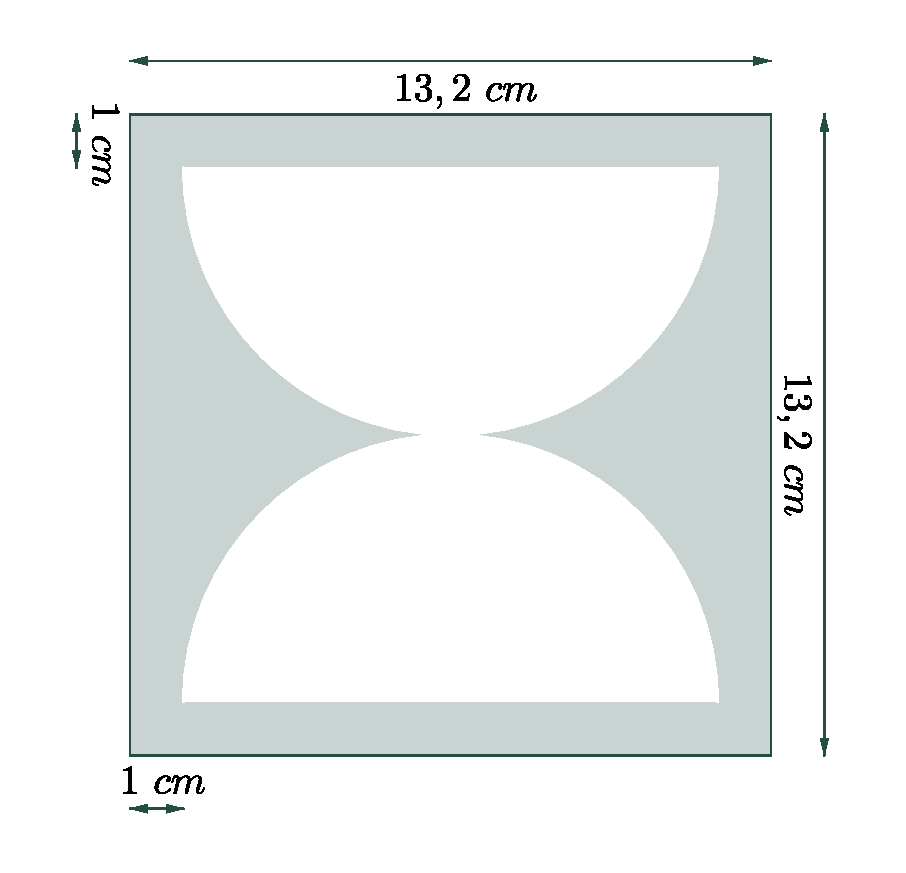
\includegraphics[width=0.9\marginparwidth]{imgc2/3-4/TK4.pdf}
        %\vspace{}
        \margincaption{Bài 17}
    \end{marginfigure}
    \xdd 
    \bt[THAM KHẢO]
    {
        Một số nơi vùng sâu vùng xa không thể đào giếng lấy nước do đụng phải đá và điều kiện đường xá hiểm trở không thể đưa máy móc vào tận nơi để khoan giếng. Nên mỗi gia đình thường xây một cái bể nước để hứng nước mưa vào mùa mưa. Đến mùa khô, sau khi dùng hết nước, người ta sẽ gánh nước từ các con suối để đổ vào bể nước.\xd 
        Một bể chứa nước của một hộ gia đình được xây bằng gạch có hình hộp chữ nhật có chiều dài $4~m$, chiều rộng $2~m$ và cao $1~m$. Gia đình có 2 người cùng gánh nước để đổ nước vào bể chứa trên. Mỗi người sử dụng hai chiếc thùng hình trụ có chiều cao $0,4~m$ và đường kính đáy $0,35~m$. Trung bình mỗi người gánh 5 chuyến trong một giờ, lượng nước khi về đến bể nước chỉ còn $90\%$. Hỏi sau bao lâu thì bể chứa sẽ đầy $50\%$ dung tích?
    }
    % Hình
    \begin{marginfigure}|-5cm|
        \centering
        \includegraphics[width=\marginparwidth]{imgc2/3-4/TK5.pdf}
        %\vspace{}
        \margincaption{Bài 18}
    \end{marginfigure}
    \xdd 
    \bt[THAM KHẢO]
    {
        Màng nhà kính Politiv-Israel là loại màng chuyên dụng để lợp mái nhà kính. Người ta muốn dùng loại màng nhà kính này để làm mái che một nhà kính trồng rau sạch có dạng nửa hình trụ đường kính đáy là $30~m$, chiều dài là $45~m$. Phần mái che gồm nửa hình trụ và hai nửa đáy hình trụ.
        \begin{enumerate}[label=\alph*)]
            \item Tính diện tích phần màng cần cho nhà trồng rau trên, biết phần vật liệu thi công bị hao phí $7\%$ diện tích nhà kính. (Kết quả làm tròn đến hàng đơn vị)
            \item Tính chi phí cần có để mua màng làm nhà kính trên biết rằng màng có khổ rộng $3,2~m$ và dài $100~m$ có giá 15000 đồng/$m^2$ (chỉ bán theo cuộn).
        \end{enumerate}
    }
    % Hình
    \begin{marginfigure}|-5cm|
        \centering
        \includegraphics[width=0.6\marginparwidth]{imgc2/3-4/TK6.pdf}
        \vspace{0.4cm}
        \margincaption{Bài 19}
    \end{marginfigure}
    \xdd 
    \bt[THAM KHẢO]
    {
        Một lon nước ngọt có dạng hình trụ có đường kính mặt trong của đáy là $6,5~cm$ chứa $355~ml$ nước ngọt. Nhà sản xuất thường đóng gói 24 lon vào một thùng carton hình hộp chữ nhật sao cho số lon ở mỗi hàng dọc, ngang bằng nhau và vừa khít thùng.
        \begin{enumerate}[label=\alph*)]
            \item Tính chiều cao của lon nước ngọt và thể tích thùng nước ngọt 24 lon, biết rằng để tránh lon vỡ do sự giãn nở vì nhiệt của chất lỏng thì phần nước ngọt chỉ chiếm $90\%$ thể tích lon (Kết quả làm tròn đến hàng đơn vị, bỏ qua phần mép nối, bề dày lớp nhôm không đáng kể).
            \item Lớp Lan dự định mua nước ngọt loại lon để liên hoan cuối năm và sử dụng loại ly thủy tinh hình trụ có dung tích chứa $310~ml$. Biết mỗi ly nước ngọt được rót đều chứa đá lạnh nên lượng nước ngọt trong ly chiếm $60\%$ dung tích ly. Hỏi lớp Lan mua 2 thùng nước ngọt thì rót được bao nhiêu ly có đá như vậy?
        \end{enumerate}
    }
\end{smallfont}
